% presentation.tex
% Complete Beamer presentation demonstrating various features
% Showcases slides, blocks, columns, lists, math, and figures

\documentclass[aspectratio=169]{beamer}

% Theme selection
\usetheme{Madrid}
\usecolortheme{dolphin}

% Packages
\usepackage{graphicx}
\usepackage{amsmath, amssymb}
\usepackage{listings}
\usepackage{tikz}
\usetikzlibrary{shapes, arrows.meta, positioning}

% Listings configuration for code
\lstset{
    basicstyle=\ttfamily\small,
    keywordstyle=\color{blue},
    commentstyle=\color{green!60!black},
    stringstyle=\color{red},
    numbers=left,
    numberstyle=\tiny,
    frame=single,
    breaklines=true
}

% Title information
\title[Deep Learning Intro]{Introduction to Deep Learning}
\subtitle{Neural Networks and Applications}
\author[J. Smith]{John Smith}
\institute[MIT]{
    Department of Computer Science\\
    Massachusetts Institute of Technology
}
\date{\today}

% Logo (uncomment if you have a logo file)
% \logo{\includegraphics[height=0.8cm]{logo.png}}

\begin{document}

% ==================== Title Slide ====================
\begin{frame}
    \titlepage
\end{frame}

% ==================== Outline Slide ====================
\begin{frame}{Outline}
    \tableofcontents
\end{frame}

% ==================== Section 1 ====================
\section{Introduction}

\begin{frame}{What is Deep Learning?}
    \begin{block}{Definition}
        Deep Learning is a subset of machine learning that uses artificial neural
        networks with multiple layers to progressively extract higher-level features
        from raw input.
    \end{block}

    \vspace{0.5cm}

    \begin{columns}[c]
        \column{0.5\textwidth}
        \textbf{Key Characteristics:}
        \begin{itemize}
            \item Multiple layers of processing
            \item Automatic feature learning
            \item End-to-end learning
            \item Hierarchical representations
        \end{itemize}

        \column{0.5\textwidth}
        \textbf{Applications:}
        \begin{itemize}
            \item Computer Vision
            \item Natural Language Processing
            \item Speech Recognition
            \item Game Playing (AlphaGo)
        \end{itemize}
    \end{columns}
\end{frame}

\begin{frame}{History of Neural Networks}
    \begin{itemize}
        \item \textbf{1943:} McCulloch-Pitts neuron model
        \item \textbf{1958:} Perceptron (Rosenblatt)
        \item \textbf{1986:} Backpropagation popularized (Rumelhart et al.)
        \item \textbf{1998:} LeNet-5 for digit recognition (LeCun)
        \item \textbf{2012:} AlexNet wins ImageNet (Krizhevsky et al.)
        \item \textbf{2017:} Transformer architecture (Vaswani et al.)
        \item \textbf{2020s:} Large Language Models (GPT, BERT, etc.)
    \end{itemize}

    \pause

    \begin{alertblock}{Key Breakthrough}
        The availability of large datasets, powerful GPUs, and improved algorithms
        led to the deep learning revolution in the 2010s.
    \end{alertblock}
\end{frame}

% ==================== Section 2 ====================
\section{Neural Network Fundamentals}

\begin{frame}{The Artificial Neuron}
    \begin{columns}[c]
        \column{0.6\textwidth}
        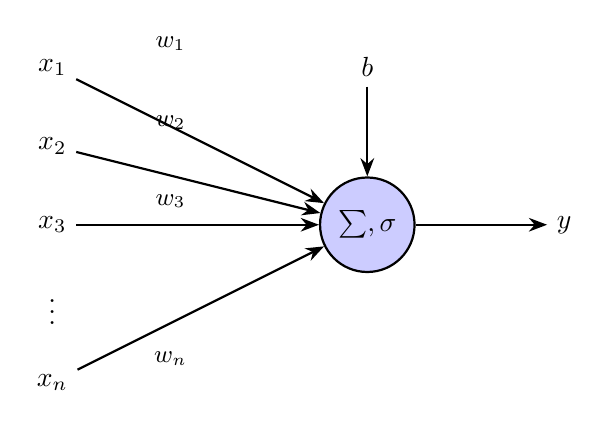
\begin{tikzpicture}[
            neuron/.style={circle, draw=black, thick, minimum size=1.2cm, fill=blue!20},
            arrow/.style={->,>=Stealth, thick}
        ]
            % Inputs
            \foreach \i in {1,2,3} {
                \node (x\i) at (0, -\i) {$x_\i$};
                \node (w\i) at (1.5, -\i+0.3) {\small $w_\i$};
            }
            \node at (0, -4) {$\vdots$};
            \node (xn) at (0, -5) {$x_n$};
            \node (wn) at (1.5, -5+0.3) {\small $w_n$};

            % Neuron
            \node[neuron] (neuron) at (4, -3) {$\sum, \sigma$};

            % Output
            \node (output) at (6.5, -3) {$y$};

            % Connections
            \foreach \i in {1,2,3} {
                \draw[arrow] (x\i) -- (neuron);
            }
            \draw[arrow] (xn) -- (neuron);
            \draw[arrow] (neuron) -- (output);

            % Bias
            \node (bias) at (4, -1) {$b$};
            \draw[arrow] (bias) -- (neuron);
        \end{tikzpicture}

        \column{0.4\textwidth}
        \textbf{Mathematical Model:}
        \begin{equation*}
            y = \sigma\left(\sum_{i=1}^{n} w_i x_i + b\right)
        \end{equation*}

        Where:
        \begin{itemize}
            \item $x_i$: inputs
            \item $w_i$: weights
            \item $b$: bias
            \item $\sigma$: activation function
        \end{itemize}
    \end{columns}
\end{frame}

\begin{frame}{Activation Functions}
    \begin{columns}[t]
        \column{0.33\textwidth}
        \centering
        \textbf{Sigmoid}
        \begin{equation*}
            \sigma(x) = \frac{1}{1 + e^{-x}}
        \end{equation*}
        \vspace{0.2cm}
        \begin{itemize}
            \item Range: (0, 1)
            \item Smooth gradient
            \item Vanishing gradient issue
        \end{itemize}

        \column{0.33\textwidth}
        \centering
        \textbf{ReLU}
        \begin{equation*}
            f(x) = \max(0, x)
        \end{equation*}
        \vspace{0.2cm}
        \begin{itemize}
            \item Range: $[0, \infty)$
            \item Most popular
            \item Computational efficiency
        \end{itemize}

        \column{0.33\textwidth}
        \centering
        \textbf{Tanh}
        \begin{equation*}
            \tanh(x) = \frac{e^x - e^{-x}}{e^x + e^{-x}}
        \end{equation*}
        \vspace{0.2cm}
        \begin{itemize}
            \item Range: (-1, 1)
            \item Zero-centered
            \item Similar issues as sigmoid
        \end{itemize}
    \end{columns}
\end{frame}

\begin{frame}[fragile]{Training Neural Networks}
    \begin{block}{Backpropagation Algorithm}
        The core algorithm for training neural networks, using gradient descent
        to minimize the loss function.
    \end{block}

    \vspace{0.3cm}

    \textbf{Key Steps:}
    \begin{enumerate}
        \item \textbf{Forward Pass:} Compute predictions
        \item \textbf{Compute Loss:} Measure error
        \item \textbf{Backward Pass:} Compute gradients
        \item \textbf{Update Weights:} Gradient descent
    \end{enumerate}

    \vspace{0.3cm}

    \begin{exampleblock}{Weight Update Rule}
        \begin{equation*}
            w_{new} = w_{old} - \eta \frac{\partial L}{\partial w}
        \end{equation*}
        where $\eta$ is the learning rate and $L$ is the loss function.
    \end{exampleblock}
\end{frame}

% ==================== Section 3 ====================
\section{Deep Learning Architectures}

\begin{frame}{Convolutional Neural Networks (CNNs)}
    \begin{columns}[c]
        \column{0.5\textwidth}
        \textbf{Key Components:}
        \begin{itemize}
            \item Convolutional layers
            \item Pooling layers
            \item Fully connected layers
        \end{itemize}

        \vspace{0.3cm}

        \textbf{Advantages:}
        \begin{itemize}
            \item Translation invariance
            \item Parameter sharing
            \item Hierarchical feature learning
        \end{itemize}

        \column{0.5\textwidth}
        \begin{center}
            \textit{[CNN Architecture Diagram]}

            \vspace{0.2cm}

            \framebox{\parbox{4cm}{
                Input Image\\
                $\downarrow$\\
                Convolution + ReLU\\
                $\downarrow$\\
                Pooling\\
                $\downarrow$\\
                Fully Connected\\
                $\downarrow$\\
                Output
            }}
        \end{center}
    \end{columns}

    \vspace{0.5cm}

    \begin{alertblock}{Applications}
        Image classification, object detection, image segmentation, face recognition
    \end{alertblock}
\end{frame}

\begin{frame}{Recurrent Neural Networks (RNNs)}
    \textbf{Designed for sequential data processing}

    \vspace{0.3cm}

    \begin{columns}[t]
        \column{0.5\textwidth}
        \textbf{Standard RNN Issues:}
        \begin{itemize}
            \item Vanishing gradients
            \item Difficulty learning long-term dependencies
            \item Limited memory
        \end{itemize}

        \vspace{0.3cm}

        \textbf{Solutions:}
        \begin{itemize}
            \item LSTM (Long Short-Term Memory)
            \item GRU (Gated Recurrent Unit)
        \end{itemize}

        \column{0.5\textwidth}
        \textbf{LSTM Advantages:}
        \begin{itemize}
            \item Cell state for long-term memory
            \item Gating mechanisms
            \item Better gradient flow
        \end{itemize}

        \vspace{0.3cm}

        \textbf{Applications:}
        \begin{itemize}
            \item Language modeling
            \item Machine translation
            \item Speech recognition
            \item Time series prediction
        \end{itemize}
    \end{columns}
\end{frame}

\begin{frame}{Transformers}
    \begin{block}{Revolutionary Architecture (2017)}
        ``Attention is All You Need'' introduced the Transformer, which replaced
        recurrence with self-attention mechanisms.
    \end{block}

    \vspace{0.3cm}

    \begin{columns}[c]
        \column{0.5\textwidth}
        \textbf{Key Innovations:}
        \begin{itemize}
            \item Self-attention mechanism
            \item Positional encoding
            \item Parallel processing
            \item Multi-head attention
        \end{itemize}

        \column{0.5\textwidth}
        \textbf{Impact:}
        \begin{itemize}
            \item BERT (2018)
            \item GPT series (2018-)
            \item Vision Transformers (2020)
            \item Foundation for modern LLMs
        \end{itemize}
    \end{columns}

    \vspace{0.3cm}

    \begin{exampleblock}{Self-Attention Formula}
        \begin{equation*}
            \text{Attention}(Q, K, V) = \text{softmax}\left(\frac{QK^T}{\sqrt{d_k}}\right)V
        \end{equation*}
    \end{exampleblock}
\end{frame}

% ==================== Section 4 ====================
\section{Practical Considerations}

\begin{frame}[fragile]{Training Best Practices}
    \begin{columns}[t]
        \column{0.5\textwidth}
        \textbf{Data Preparation:}
        \begin{itemize}
            \item Data augmentation
            \item Normalization
            \item Train/validation/test split
            \item Handling imbalanced datasets
        \end{itemize}

        \vspace{0.3cm}

        \textbf{Hyperparameters:}
        \begin{itemize}
            \item Learning rate
            \item Batch size
            \item Number of epochs
            \item Network architecture
        \end{itemize}

        \column{0.5\textwidth}
        \textbf{Regularization:}
        \begin{itemize}
            \item Dropout
            \item L1/L2 regularization
            \item Batch normalization
            \item Early stopping
        \end{itemize}

        \vspace{0.3cm}

        \textbf{Optimization:}
        \begin{itemize}
            \item Adam optimizer
            \item Learning rate scheduling
            \item Gradient clipping
            \item Mixed precision training
        \end{itemize}
    \end{columns}
\end{frame}

\begin{frame}[fragile]{PyTorch Example}
    \begin{lstlisting}[language=Python]
import torch
import torch.nn as nn

class SimpleNN(nn.Module):
    def __init__(self):
        super(SimpleNN, self).__init__()
        self.fc1 = nn.Linear(784, 256)
        self.fc2 = nn.Linear(256, 128)
        self.fc3 = nn.Linear(128, 10)
        self.relu = nn.ReLU()

    def forward(self, x):
        x = x.view(-1, 784)  # Flatten
        x = self.relu(self.fc1(x))
        x = self.relu(self.fc2(x))
        x = self.fc3(x)
        return x
    \end{lstlisting}
\end{frame}

% ==================== Section 5 ====================
\section{Conclusion}

\begin{frame}{Summary}
    \begin{block}{What We Covered}
        \begin{itemize}
            \item Fundamentals of neural networks
            \item Major deep learning architectures (CNN, RNN, Transformer)
            \item Training algorithms and best practices
            \item Practical implementation considerations
        \end{itemize}
    \end{block}

    \vspace{0.5cm}

    \begin{exampleblock}{Key Takeaways}
        \begin{enumerate}
            \item Deep learning has revolutionized AI
            \item Architecture choice depends on the problem domain
            \item Proper training requires careful hyperparameter tuning
            \item Transformers are the current state-of-the-art for many tasks
        \end{enumerate}
    \end{exampleblock}
\end{frame}

\begin{frame}{Future Directions}
    \begin{columns}[c]
        \column{0.5\textwidth}
        \textbf{Research Trends:}
        \begin{itemize}
            \item Scaling laws
            \item Multimodal models
            \item Efficient architectures
            \item Neural architecture search
            \item Explainable AI
        \end{itemize}

        \column{0.5\textwidth}
        \textbf{Challenges:}
        \begin{itemize}
            \item Computational costs
            \item Data requirements
            \item Bias and fairness
            \item Robustness
            \item Interpretability
        \end{itemize}
    \end{columns}

    \vspace{0.5cm}

    \begin{alertblock}{The Future is Bright}
        Deep learning continues to advance rapidly, with new breakthroughs
        happening regularly. Stay curious and keep learning!
    \end{alertblock}
\end{frame}

\begin{frame}[standout]
    \Huge Thank You!

    \vspace{1cm}

    \Large Questions?

    \vspace{1cm}

    \normalsize
    Contact: john.smith@mit.edu
\end{frame}

% ==================== Backup Slides ====================
\appendix

\begin{frame}{Additional Resources}
    \textbf{Books:}
    \begin{itemize}
        \item Deep Learning (Goodfellow, Bengio, Courville)
        \item Neural Networks and Deep Learning (Nielsen)
        \item Dive into Deep Learning (Zhang et al.)
    \end{itemize}

    \vspace{0.3cm}

    \textbf{Online Courses:}
    \begin{itemize}
        \item Stanford CS231n (Computer Vision)
        \item Stanford CS224n (NLP)
        \item fast.ai Practical Deep Learning
    \end{itemize}

    \vspace{0.3cm}

    \textbf{Frameworks:}
    \begin{itemize}
        \item PyTorch: \url{https://pytorch.org}
        \item TensorFlow: \url{https://tensorflow.org}
    \end{itemize}
\end{frame}

\end{document}
